\subsection{Topología ferroviaria original}

	El primer ejemplo, ilustrado en la Figura \ref{fig:EJ1_1}, es una topología diseñada en base a dos líneas principales y tres niveles de ramificaciones. La primera ramificación, utilizando el cambio de vías Sw06, es una ramificación simple. La segunda ramificación, utilizando el cambio de vías Sw04, es una ramificación compleja al incluir el cambio de vías Sw07 a continuación. Ademas, se incluyeron los cambios de vías Sw12 y Sw13 para permitir el intercambio de formaciones entre ambas vías principales. El objetivo de este ejemplo fue comprobar el funcionamiento del RNA con una topología de múltiples ramificaciones anidadas.	
	
	\begin{figure}[h]
		\centering
		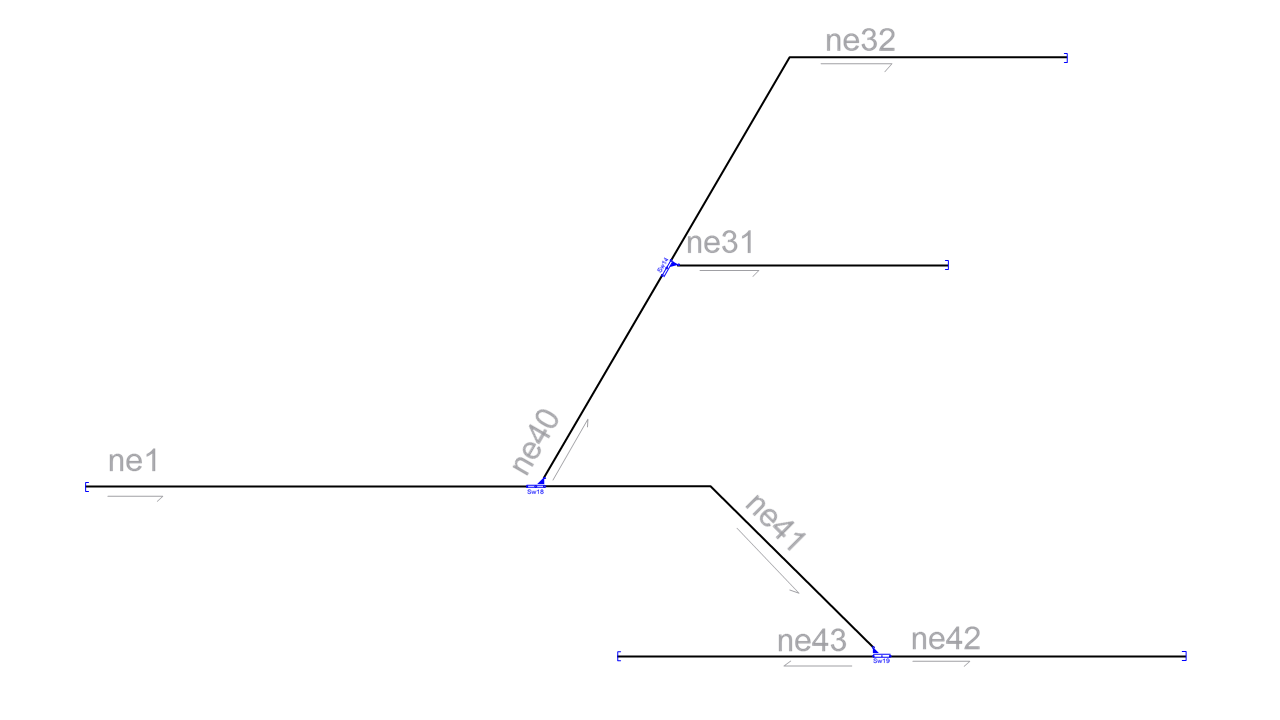
\includegraphics[width=1\textwidth]{resultados-obtenidos/ejemplo7/images/7_empty.png}
		\centering\caption{Topología ferroviaria del ejemplo 7 sin señalamiento.}
		\label{fig:EJ7_1}
	\end{figure}
	
	Para incrementar la dificultad del análisis y obtener resultados mas completos, se incluyeron finales de vías relativos y absolutos, junto con plataformas (Plat11, Plat13) y cruces de vías (Lc06, Lc08). La infraestructura se distribuyó de forma tal de tener que en algunos casos el espacio entre ambos fuese suficiente (Lc06 6 y Plat11) y en otros no (Lc08 y Plat13).